\documentclass[10pt]{article}
\usepackage{amssymb,amsmath,times,url,graphicx,amsthm,alltt}
%\usepackage[pdftex,urlcolor=blue,pdfpagemode=none,pdfstartview=FitH]{hyperref}
\usepackage{my_packages}
\usepackage{tikz_packages}
%% url smaller font.
\makeatletter
\def\url@leostyle{%
  \@ifundefined{selectfont}{\def\UrlFont{\sf}}{\def\UrlFont{\small\ttfamily}}}
\makeatother
\urlstyle{leo}

%\usepackage[all,import]{xy}

\renewcommand{\baselinestretch}{1.2}
\date{}

\renewcommand{\thesubsection}{\arabic{subsection}. }
\renewcommand{\thesubsubsection}{\arabic{subsection}.\arabic{subsubsection} }

\theoremstyle{definition}
\newtheorem{prob}{Problem}[section]
%\renewcommand{\theprob}{\arabic{section}.\arabic{prob}}
\renewcommand{\theprob}{\arabic{prob}}

\newenvironment{subprob}%
{\renewcommand{\theenumi}{\alph{enumi}}\renewcommand{\labelenumi}{(\theenumi)}\begin{enumerate}}%
{\end{enumerate}}%

\newenvironment{matlab}
{\begin{alltt}\small\renewcommand{\baselinestretch}{1.2}\selectfont}%
{\end{alltt}}


\begin{document}



\setcounter{page}{1}
\pagestyle{plain}
\section*{MAE3145: Homework 4}
\vspace*{-0.4cm}
\noindent{Due date: \SI{2458038.1979166665}{\julianday} }%\\%\vspace*{0.5cm}

\begin{prob}
    Halley's comet last passed through perihelion on Feb 9, 1986.
    The orbit is described with an eccentricity of \( e = 0.9671429\) and a semi-major axis of \( a = 17.834144 \si{\astronomicalunit} \).
    In 1986, the European Space Agency spacecraft Giotto encountered and photographed teh nucleus of the comet as it approached the Sun.
    Data from Giotto's camera was used to generate the enhanced image shown in~\cref{fig:halley}.
    \begin{figure}[htbp]
        \centering
        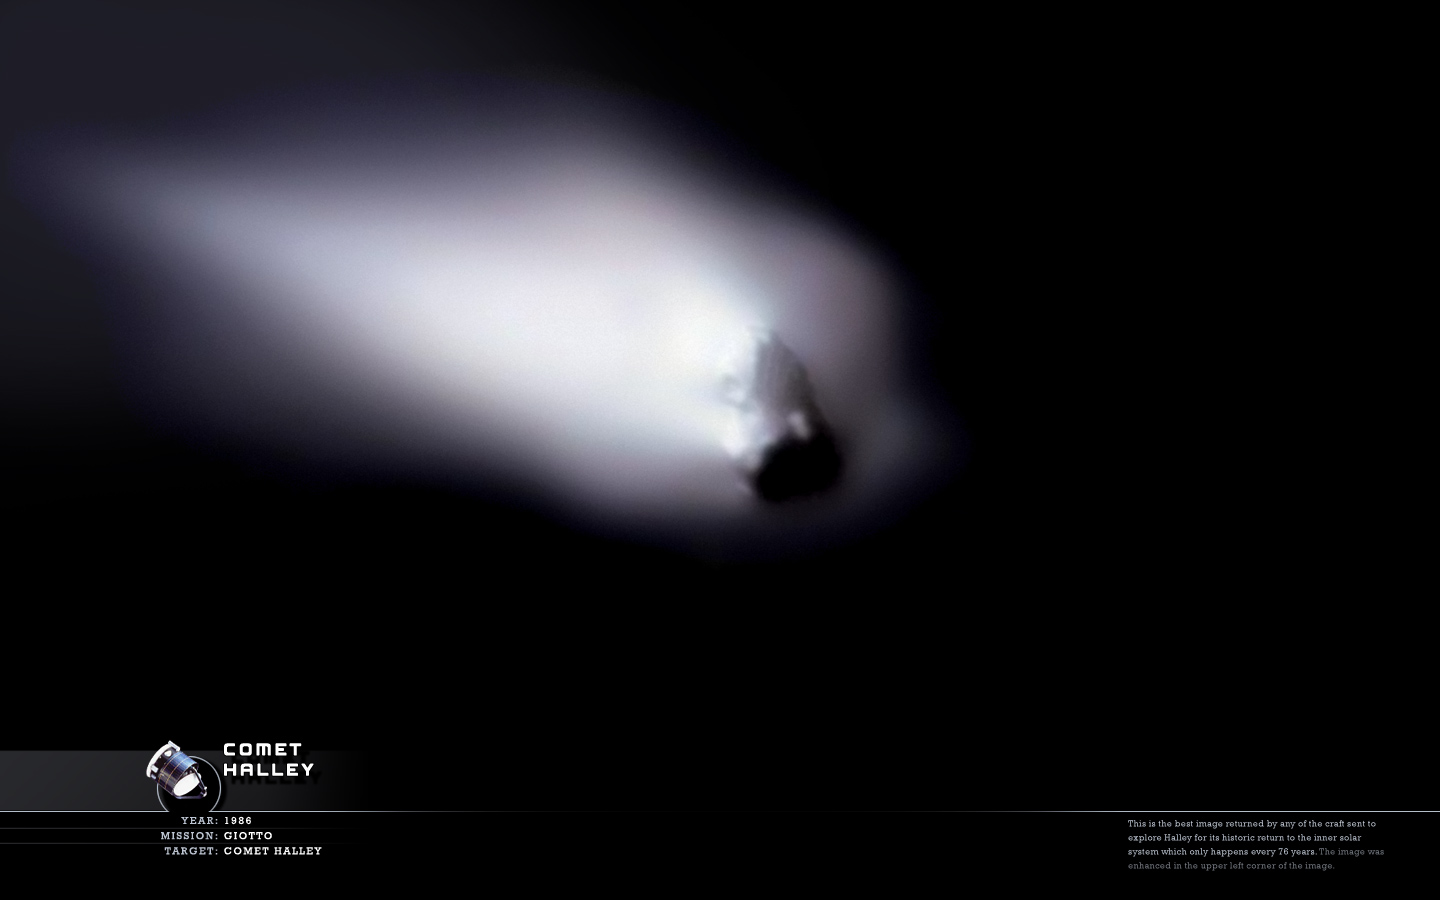
\includegraphics[width=0.75\textwidth, keepaspectratio]{figures/halley.jpg}
        \caption{Halley's Comet as seen by Giotto\label{fig:halley}}
    \end{figure}
    The potatoe shaped nucleus measures roughly \SI{15}{\kilo\meter} across and is composed primarily of water and carbon dioxide ices.

    \begin{subprob}
    \item On this date, determine the following additional orbital characteristics associated with Halley's orbit (assume a conic model):
        \begin{align*}
            r, \quad v, \quad \nu, \quad \gamma, \quad \mathcal{E}, \quad h, \quad \mathsf{P}, \quad r_a, \quad r_p, \quad E
        \end{align*}
        Ensure that you list all distances in astronomical units.
    \end{subprob}

    You can check the path of 1P/Halley at the JPL Small-Body Data Browser by going to the following \href{https://ssd.jpl.nasa.gov/sbdb.cgi?ID=c00001_0}{link}.
        Observers on Earth can pick up the comet when its true anomaly is approximately \SI{100}{\degree} prior perihelion.
    \begin{subprob}
    \item Determine the same quantities shown in part (a) above, but at the time when the observers expect to pick up the next return.
    \item Determine the time required to go from the last perihelion passage to the location where Earth observers can again pick up the return of Halley's Comet.
        What is the approximate date?
        How old will you be?
    \item How many days until the comet passes through perihelion?
\end{prob}

\begin{prob}
    A satellite is in orbit about the Earth. 
    Assume that it is reasonable to model the behavior in terms of the relative two-body problem (Earth and Satellite).
    The orbit is characterized by \( r_p = 1.5 R_{\bigoplus} \) and \( r_a = 6.2 R_{\bigoplus} \).
    It is currently located, \( t_0 \), at the point in the orbit such that \( \nu = \SI{135}{\degree} \).

    \begin{subprob}
        \item Determine the following orbit paramterts and satellite state information:
            \begin{align*}
                a, \quad e, \quad p, \quad \mathsf{P}, \quad \mathcal{E}, \quad r_0, \quad v_0, \quad E_0, \quad \gamma_0, \quad \parenth{t_0 - T}.
            \end{align*}
            List the time in hours and all angles in degrees.
        \item Write \( \bar r_0, \bar v_0 \) in terms of components in both the local vertical/local horizontal and perifocal reference frames.
        \item Determine the value of true anomaly in exactly \SI{3}{\hour}.
            Determine the satellite state at the new time, \( t_1 \).
            \begin{align*}
                r_1, \quad v_1, \quad E_1, \quad \gamma_1, \parenth{t_1 - T}
            \end{align*}
            Determine the \( \Delta \nu, \Delta E \) that corresponds to \( \Delta t = \SI{3}{\hour} \).
        \item Write \( \bar r_1, \bar v_1 \) in terms of the local vertical/local horizontal and perifocal reference frames.
        \item Plot the orbit using your skills from the previous homeworks.
            By hand, mark on the plot the location of perigee and location of the satellite at \( t_0 \) and \( t_1 \). 
            At each location indicate \( r, \nu, \bar v, E, \gamma \) also sketch the local horizon.
            Add the auxillary circle and mark \( \Delta \nu \) and \( \Delta E \).
    \end{subprob}
\end{prob}

\begin{prob}
    As part of some interplanetary mission, assume that a spacecraft departs the Earth vicinity along a hyperbola.
    The hyperbola is defined such that \( r_p = \SI{1000}{\kilo\meter} \) and \( e  = 1.05\).

    \begin{subprob}
        \item Determine the following orbital characteristics: \( a, p, v_\infty, \mathcal{E}, \delta, \nu_\infty \) and the aiming radius.
        \item When the spacecraft reaches \( \nu_1 = \SI{90}{\degree} \), determine \( r_1, v_1, H_1, \gamma_1, \parenth{t_1 - T } \).
            Write \( \bar r_1, \bar v_1 \) in terms of the local vertical/local horizontal and perifocal reference frames?
        \item Plot the hyperbolic orbit between \( \pm \SI{135}{\degree} \), ensure you also include asymptotes.
            Label the appropriate quantities including, \( b, \delta, \frac{\delta}{2} , \nu_\infty, a, \gamma, \text{center} , \text{local horizon} \).
            Add the Earth to scale.
        \item How long until the spacecraft reaches \( \nu_2 = \SI{150}{\degree} \), \( t = t_2\)?
            What is the value of \( r \) at this time?
    \end{subprob}
\end{prob}

\begin{prob}
    An orbit transfer vehicle (OTV) is currently in Earth orbit with the following characteristics ( with respect to the Earth Centered Inertial frame).
    \begin{align*}
        a &= 3 R_{\oplus} \qquad \Omega = \SI{45}{\degree} \\
        e &= 0.40 \qquad \omega = \SI{90}{\degree} \\
        i &= \SI{28.5}{\degree} \qquad \nu = \SI{235}{\degree}
    \end{align*}

    \begin{subprob}
    \item Determine the state of the satellite and additional orbital parameters: \( \bar r, \bar v, r, v, \gamma, \nu, M , E, \parenth{t - T}\).
        In addition, write \( \bar r, \bar v \) in terms of the local horizontal/local vertical, perifocal, and inertial reference frames.
    \item Plot the orbital plane and mark all of the appropriate quantities.
        What are the appropriate quantities?
    \end{subprob}
\end{prob}

\begin{prob}
    The OTV is now in a new orbit.
    At a certain time, the following information is given.
    \begin{align*}
        \bar r_1 &= 3.0 R_\oplus \hat x + 5.0 R_\oplus \hat y \, \si{\kilo\meter}\\
        \bar v_1 &= -3.2 \hat x + 2.0 \hat y + 2.5 \hat z \, \si{\kilo\meter\per\second} .
    \end{align*}

    Determine the following and plot the orbit in the orbital plane.

    \begin{align*}
        a, \quad e, \quad i, \quad \omega, \quad \Omega, \quad r, \quad v, \quad \gamma, \quad \nu, \quad M, \quad E, \quad \parenth{t - T}.
    \end{align*}
\end{prob}
\end{document}


